\newcommand{\multivar}{/home/robin/ENSEIGN/Cours/MathBiologie/L3-ENS-Math1/Exercices/MultiVar}

%-------------------------------------------------------------------------------
\subsection{Normes}
%-------------------------------------------------------------------------------

%-------------------------------------------------------------------------------
\subsubsection{Equivalence des normes}
%-------------------------------------------------------------------------------

Donner des constantes $c_1$ et $c_2$ permettant de comparer les trois normes $\|\cdot\|_1$, $\|\cdot\|_2$ et $\|\cdot\|_\infty$ dans $\Rbb^n$.
\solution{On considère les trois paires de normes.
\begin{description}
  \item[$\|x\|_2$ et $\|x\|_\infty$:] On a vu en cours que
  $$
  \|x\|_\infty \leq \|x\|_2 \leq \sqrt{n} \|x\|_\infty.
%   \qquad \Rightarrow \qquad
%   \frac1{\sqrt{n}} \|x\|_2 \leq \|x\|_\infty \leq \|x\|_2. 
  $$
  \item[$\|x\|_1$ et $\|x\|_\infty$:]  On voit facilement que 
  $$
  \|x\|_\infty \leq \|x\|_1 \leq n \|x\|_\infty.
%   \qquad \Rightarrow \qquad
%   \frac1n \|x\|_1 \leq \|x\|_\infty \leq \|x\|_1.
  $$
  \item[$\|x\|_1$ et $\|x\|_2$:]  On peut déduire une comparaison de $\|x\|_1$ et $\|x\|_2$ en combinant ces résultats
  \begin{align*}
  & \|x\|_1 \leq n \|x\|_\infty \leq n \|x\|_2 \leq n^{3/2} \|x\|_\infty \leq n^{3/2} \|x\|_1 \\
  \Rightarrow \qquad
  & \frac1n \|x\|_1 \leq \|x\|_2 \leq \sqrt{n} \|x\|_1.
%   \Rightarrow \qquad
%   & \frac1{\sqrt{n}} \|x\|_2 \leq \|x\|_1 \leq n \|x\|_2.
  \end{align*}
  On peut cependant affiner les deux constantes :
  \begin{description}
    \item[$\|x\|_2 \leq c_1 \|x\|_1$ :] en définissant, pur $1 \leq i \leq n$, les vecteurs $u_i = x_i e_i$ (où les $e_i$ sont les vecteurs de la base canonique), l'inégalité triangulaire pour la norme $\|\cdot\|_2$ implique que
    $$
    \|x\|_2 \leq \sum_i \|u_i\|_2 = \sum_i |x_i| = \|x\|_1 ;
    $$
    \item[$\|x\|_1 \leq c_2 \|x\|_2$ :] en utilisant le fait que $2ab \leq a^2 + b^2$, il vient
%     la boule unité de la norme $\|\cdot\|_2$ est incluse dans la boule de rayon $\sqrt{n}$ de la norme $\|\cdot\|_1$, il vient que $\|x\|_1 \leq \sqrt{n} \|x\|_2$.
    \begin{align*}
      \|x\|_1^2
      & = \left(\sum_i |x_i|\right)^2
      =  \sum_i |x_i|^2 + \sum_{i < j} 2 |x_i||x_j| \\ 
      & \leq \sum_i |x_i|^2 + \sum_{i < j} (|x_i|^2 + |x_j|^2) 
      = \sum_i |x_i|^2 + \sum_{i \neq j} |x_i|^2 \\
      & = n \sum_i |x_i|^2 = n \|x\|_2^2,
    \end{align*}
    c'est-à-dire : $\|x\|_1 \leq \sqrt{n} \|x\|_2$ ;
  \end{description}
  soit au total
  $$
  \frac1{\sqrt{n}} \|x\|_1 \leq \|x\|_2 \leq \|x\|_1.
  $$
\end{description}
On peut vérifier que les constantes sont optimales en donnant des exemples pour lesquels chacune des égalités est obtenue. Considérons le vecteur $x$ dont toutes les coordonnées sont égales et le vecteur $y$ dont toutes les coordonnées sont nulles, sauf une (par exemple, la première) :
$$
x = a 1_n, \qquad y = b e_1.
$$
On a :
\begin{align*}
  & \text{pour } \|\cdot\|_2 \text{ et } \|\cdot\|_\infty : & 
  \|x\|_2 & = \sqrt{n} \|x\|_\infty, & 
  \|y\|_2 & = \|y\|_\infty; \\
  & \text{pour } \|\cdot\|_1 \text{ et } \|\cdot\|_\infty : & 
  \|x\|_1 & = n \|x\|_\infty, & 
  \|y\|_1 & = \|y\|_\infty; \\
  & \text{pour } \|\cdot\|_1 \text{ et } \|\cdot\|_2 : & 
  \|y\|_2 & = \|y\|_1, &
  \|x\|_1 & = \sqrt{n} \|x\|_2.
\end{align*}
}



%-------------------------------------------------------------------------------
\subsubsection{Norme fondée sur une matrice définie positive}
%-------------------------------------------------------------------------------

  Soit $A$ une matrice de $\Mcal_n$ symétrique définie positive (strictement): $A \succ 0$. Montrer que $\|\cdot\|_A$ définie par $\|x\|_A = (x^\top A x)^{1/2}$ est une norme pour $\Rbb^n$.
\solution{On vérifie les 3 conditions définissant une norme.
  \begin{enumerate}
   \item Par définition des matrices définies positives, on a bien pour tout $x \in \Rbb^n$, $x^\top A x \geq 0$  et $\{x^\top A x = 0\} \Leftrightarrow \{x = 0\}$.
   \item On a également $\|\lambda x\|_A = ((\lambda x)^\top A (\lambda x))^{1/2} = (\lambda^2 x^\top A x)^{1/2} = |\lambda| \|x\|_A$ ;
   \item Puisque $A$ est symétrique, on a
   $$
   \|x + y\|^2_A 
   = \|x\|^2_A + \| y\|^2_A + 2 x^\top A y
   $$
   et on peut la décomposer sous la forme $A = P \Lambda P^\top$ où $P$ et $P^\top$ sont orthonormales. Posons $u = \Lambda^{1/2} P^\top x$ et $v = \Lambda^{1/2} P^\top y$ qui vérifient
   \begin{align*}
   \|u\|_2 & = \sqrt{x^\top P \Lambda^{1/2} \Lambda^{1/2} P^\top x} = \|x\|_A, & 
   \|v\|_2 & = \|y\|_A, \\
   x^\top A y & = u^\top v.
   \end{align*}
   Par Cauchy-Schwarz, on a alors
   \begin{align*}
    \|x + y\|^2_A 
    & = \|u\|^2_2 + \|v\|^2_2 + 2 u^\top v \leq \|u\|^2_2 + \|v\|^2_2 + 2 |u^\top v| \\
    & \leq \|u\|^2_2 + \|v\|^2_2 + 2 \|u\|_2 \|v\|_2 = (\|u\|_2 + \|v\|_2)^2 \\
    & = (\|x\|_A + \|y\|_A)^2.    
   \end{align*}
  \end{enumerate}
}



%-------------------------------------------------------------------------------
\subsection{Application linéaire tangente}
%-------------------------------------------------------------------------------

%-------------------------------------------------------------------------------
\subsubsection{Cube d'une matrice}
%-------------------------------------------------------------------------------

Soit la fonction
$$
\begin{array}{rrcl}
  f :  & \Mcal_n(\Rbb) & \mapsto & \Mcal_n(\Rbb) \\
  & X & \rightarrow & X^3.
\end{array}
$$
Démontrer qu'elle est partout différentiable et déterminer son application linéaire tangente $D_X f$ en toute matrice $X$ de $\Mcal_n(\Rbb)$.
\solution{
  On a
  $$
  f(X+H) = X^3 + X^2H + XHX + HX^2 + H^2X + HXH + XH^2 + H^3.
  $$
  Comme pour la fonction $f(X) = X^2$, on montre que 
  $$
  H^2X = o(\|H\|), \qquad HXH  = o(\|H\|), \qquad XH^2  = o(\|H\|), \qquad H^3 = o(\|H\|).
  $$
  On a donc 
  $$
  f(X+H) - f(X) = X^2H + XHX + HX^2 + o(\|H\|)
  $$
  où $X^2H + XHX + HX^2$ est linéaire en $H$. L'application linéaire tangente est donc
  $$
  \begin{array}{rrcl}
    L_X : & \Mcal_n(\Rbb) & \mapsto & \Mcal_n(\Rbb) \\
    & H & \rightarrow & X^2H + XHX + HX^2.
  \end{array}
  $$
}


%-------------------------------------------------------------------------------
\subsubsection{Application linéaire tangente à une forme quadratique} 
%-------------------------------------------------------------------------------

On considère une matrice $A \in \Mcal_n$ symétrique, un vecteur $v \in \Rbb^n$ et la fonction 
$$
\begin{array}{rlll}
  f : & \Rbb^n & \mapsto & \Rbb \\
  & x & \to & f(x) = x^\top A x + v^\top x.
\end{array}
$$

\begin{enumerate}
  \item Montrer qu'il existe un vecteur $g(x) \in \Rbb^n$, qu'on précisera, tel que l'application linéaire tangente à $f$ en $x$ s'écrit
  $$
  \begin{array}{rlll}
    D_xf : & \Rbb^n & \mapsto & \Rbb^n \\
    & h & \to & D_xf(h) = g(x)^\top h.
  \end{array}
  $$
  \solution{On écrit
  \begin{align*}
    f(x+h) 
    & = (x+h)^\top A (x+h) + v^\top (x+h)
    = f(x) + x^\top A h + h^\top A x + h^\top A h + v^\top h \\
    & = f(x) + (2 x^\top A + v^\top) h + h^\top A h
  \end{align*}
  puisque $x^\top A h = h^\top A x$. On remarque alors que $h^\top A h = o(\|h\|)$ pour conclure que, puisque $A$ est symétrique, l'application linéaire tangent $D_x f$ s'écrit bien
  $$
  D_xf(h) = g(x)^\top h
  \qquad \text{avec} \quad
  g(x) = 2 A x + v.
  $$}
  \item En supposant que $A$ est inversible, déterminer le point stationnaire $x^*$ où $g(x)$ s'annule.
  \solution{En supposant $A$ inversible, on a
  $$
  g(x^*) = 0
  \qquad \Leftrightarrow \qquad
  2 A x^* + v = 0
  \qquad \Leftrightarrow \qquad
  x^* = - \frac12 A^{-1} v.
  $$}
  \item Donner une condition sur$A$ pour que $A$ soit un minimum local. (On pourra calculer la matrice hessienne de $A$.)
  \solution{La matrice hessienne de l'application $f$ en tout point $x$ vaut $H_x = 2 A$ (il suffit de déterminer l'application linéaire tangente à $g(x)$).
  $x^*$ est donc un minimum ssi $A$ est strictement définie négative}
  \item Discuter l'utilité de l'hypothèse selon laquelle $A$ est symétrique.
  \solution{On peut décomposer $A$ en ses parties symétrique $S$ et anti-symétrique $T$ : 
  $$
  S = \frac12(A + A^\top), \qquad 
  T = \frac12(A - A^\top), \qquad 
  \Rightarrow \quad
  A = S + T
  $$
  et remarquer que
  $$
  f(x) 
  = x^\top A x + v^\top x
  = x^\top S x + \frac12 \underset{=0}{\underbrace{(x^\top A x - x^\top A^\top x)}} + v^\top x,  
  $$
  c'est-à-dire que seulle la partie symétrique de $A$ contribue à la fonction Ode $f$.}
\end{enumerate}




%-------------------------------------------------------------------------------
\subsection{Matrice jacobienne}
%-------------------------------------------------------------------------------

%-------------------------------------------------------------------------------
\subsubsection{Jacobienne de $F \circ F$}
%-------------------------------------------------------------------------------

On considère une fonction 
$$
\begin{array}{rrcl}
  F : & [0, 1] \times [0, 1] & \mapsto & [0, 1] \times [0, 1] \\
  & (x, y) & \to & F(x, y) = (f_1(x, y), f_2(x, y))
\end{array}
$$
\begin{enumerate}
  \item \'Ecrire la matrice jacobienne $J(x, y)$ de la fonction $F$ en tout $(x, y) \in [0, 1] \times [0, 1]$.
  \solution{Par définition, on a
  $$
  J_{(x, y)} F = \left[\begin{array}{cc}
                        f'_{1x}(x, y) & f'_{1y}(x, y) \\
                        f'_{2x}(x, y) & f'_{2y}(x, y)
                       \end{array}\right] 
                       \qquad \text{où} \quad 
  f'_{1x}(x, y) = \left.\frac{\partial f_1}{\partial x}\right|_{(x, y)}.
  $$
  }
  \item \'Ecrire l'application linéaire tangente de $F \circ F$ en tout point $(x, y)$.
  \solution{Par définition, on a
  \begin{align*}
    J_{(x, y)} F \circ F 
    & = J_{(x, y)} F \cdot J_{F(x, y)} F \\
    & = \left[\begin{array}{cc}
          f'_{1x}(x, y) & f'_{1y}(x, y) \\
          f'_{2x}(x, y) & f'_{2y}(x, y)
        \end{array}\right]
        \left[\begin{array}{cc}
          f'_{1x}(F(x, y)) & f'_{1y}(F(x, y)) \\
          f'_{2x}(F(x, y)) & f'_{2y}(F(x, y))
        \end{array}\right].
  \end{align*}
  L'application linéaire tangente au point $(x^*, y^*)$ est donc
  \begin{align*}
  L_{(x^*, y^*)}(x, y) 
  & = F(F(x^*, y^*)) \\
  & \qquad + (f'_{1x}(x^*, y^*) f'_{1x}(F(x^*, y^*)) + f'_{1y}(x^*, y^*) f'_{2x}(F(x^*, y^*))) x \\
  & \qquad +(f'_{2x}(x^*, y^*) f'_{1y}(F(x^*, y^*)) + f'_{2y}(x^*, y^*) f'_{2y}(F(x^*, y^*))) y 
  \end{align*}}
  \item On suppose que $F(1, 1) = (1, 1)$. Donner la matrice jacobienne $J_n(1, 1)$ de la fonction $F$ itérée $n$ fois avec elle-même, en $(x, y) = (1, 1)$.
  \solution{On a alors $J_{F(1, 1)}F = J_{(1, 1)}F$, soit
  $$
  J_2(1, 1)
  = J_{(1, 1)} F \circ F 
  = J_{(1, 1)} F \cdot J_{F(1, 1)} F 
  = \left(J_{(1, 1)} F\right)^2.
  $$
  Par récurrence, puisque
  $$
  J_{(x, y)} F^n 
  = J_{(x, y)} (F^{n-1} \circ F)
  = J_{(x, y)} F \cdot J_{F(x, y)} F^{n-1},
  $$
  il vient
  $$
  J_n(1, 1) = \left(J_{(1, 1)} F\right)^n.
  $$
  }
\end{enumerate}




%-------------------------------------------------------------------------------
\subsection{Extrema}
%-------------------------------------------------------------------------------

%-------------------------------------------------------------------------------
\subsubsection{Exemple de fonction de $\Rbb^2 \mapsto \Rbb$}
%-------------------------------------------------------------------------------

Soit la fonction $f: \Rbb^2 \mapsto \Rbb$ définie par
$$
f(x, y) = x^3 + y^3 - 3 xy
$$

\begin{enumerate}
  \item Déterminer les points stationnaires de la fonction $f$.
  \solution{
    Le gradient de $f$ vaut
    $$
    \nabla f = \left[\begin{array}{c} 3x^2 - 3y \\ 3y^2 - 3x \end{array}\right]
    $$
    qui est nul aux points
    $$
    a = (0, 0) \qquad \text{et} \qquad b = (1, 1).
    $$
  }
  \item Déterminer s'il s'agit de maximums, de minimums ou de points selles.
  \solution{
    La hessienne vaut
    $$
    \nabla^2 f = \left[\begin{array}{rrr} 6x & & -3 \\ -3 & & 6y \end{array}\right].
    $$
    \begin{description}
      \item[\'Etude du point $a$ :] on a 
      $$
      \nabla_a^2 f = \left[\begin{array}{rrr} 0 & & -3 \\ -3 & & 0 \end{array}\right]
      \qquad \Rightarrow \qquad 
      | \nabla_a^2 f | = -9 < 0
      $$
      donc $a$ est un point selle. Ses valeurs propres sont les racines de
      $$
      P(\lambda) = \left|\begin{array}{rrr} -\lambda & & -3 \\ -3 & & -\lambda \end{array}\right|
      = \lambda^2 - 9 
      \qquad \text{soit} \quad 
      \lambda = \pm 3.
      $$
      Tout vecteur propre associé à $\lambda = -3$ est solution de 
      $$
      \left\{\begin{array}{rcl} -3y & = & -3x \\-3x & = & -3y\end{array} \right.
      \qquad \Rightarrow \qquad 
      x = y
      \qquad \Rightarrow \qquad 
      \left[ \begin{array}{r} 1 \\ 1 \end{array} \right] \text{ est associé à $-3$}
      $$
      donc $a$ est un maximum dans la direction de la 1ère bissectrice. \\
      Tout vecteur propre associé à $\lambda = 3$ est solution de 
      $$
      \left\{\begin{array}{rcl} -3y & = & 3x \\-3x & = & 3y\end{array} \right.
      \qquad \Rightarrow \qquad 
      x = -y
      \qquad \Rightarrow \qquad 
      \left[ \begin{array}{r} -1 \\ 1 \end{array} \right] \text{ est associé à $+3$}
      $$
      donc $a$ est un minimum dans la direction de la 2ème bissectrice.
      $$
      \begin{tabular}{cc}
        direction $x = y$ & direction $x = -y$ \\
        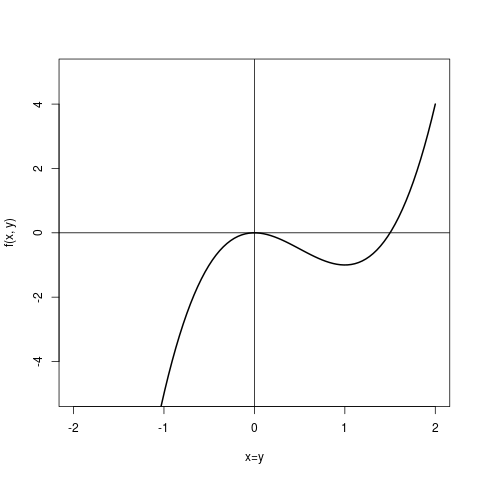
\includegraphics[width=.35\textwidth, trim=00 10 10 40, clip=]{ExempleOptimum-1ereBissectrice} &
        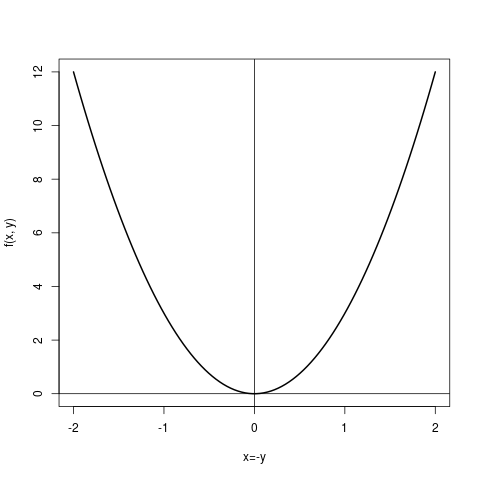
\includegraphics[width=.35\textwidth, trim=00 10 10 40, clip=]{ExempleOptimum-2emeBissectrice} \\
        $f(x, x) = 2x^3 - 3x^2$ & $f(x, -x) = 3x^2$
      \end{tabular}
      $$
      \item[\'Etude du point $b$ :] on a
      $$
      \nabla_b^2 f = \left[\begin{array}{rrr} 6 & & -3 \\ -3 & & 6 \end{array}\right]
      \qquad \Rightarrow \qquad 
      | \nabla_b^2 f | = 27 > 0, \qquad \tr(\nabla_b^2 f) = 12 > 0
      $$
      donc les deux valeurs propres de $\nabla_b^2 f$ sont positives : $b$ est donc un minimum.
    \end{description}
    Au total la surface d'équation $\{z = f(x, y)\}$ a l'aspect suivant
    $$
    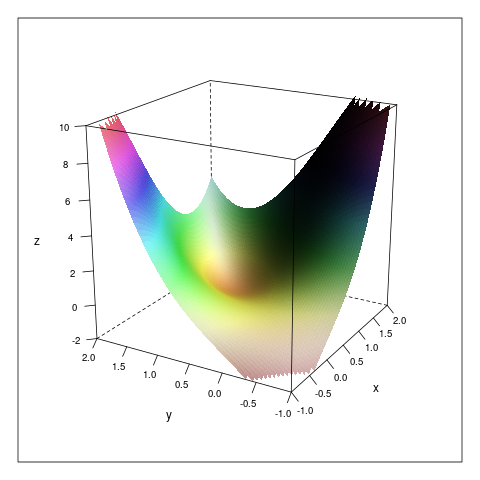
\includegraphics[width=.6\textwidth]{ExempleOptimum-surface}
    $$
  }
\end{enumerate}



% Voir \url{www.bibmath.net/ressources/index.php?action=affiche&quoi=bde/analyse/calculdiff/extrema&type=fexo}, exercice 7 (en fait, bof : un peu long)

Voir \url{www.bibmath.net/ressources/index.php?action=affiche&quoi=bde/analyse/calculdiff/extrema&type=fexo}, exercice 16
